\subsection{H-brygga}
För att styra hastighet och riktning av framdrivningsmotorerna designades en h-brygga för att kunna leverera 12V 3A. Design och tester för h-bryggan arbetades fram parallellt med ett projekt i en annan kurs (TNE089 - Elektromagnetisk kompatibilitet och mönsterkortdesign) för en grundlig design. För en mer utförlig rapport om h-bryggans design finns rapporten från TNE089 i Appendix.

\subsubsection{Resultat}
Ett kretsschema designades med Altium Designer 6, kretsschemat kan ses i figur \ref{fig:h_brygga_schema}.

\begin{landscape}
\begin{figure}[htbp!]
\centering
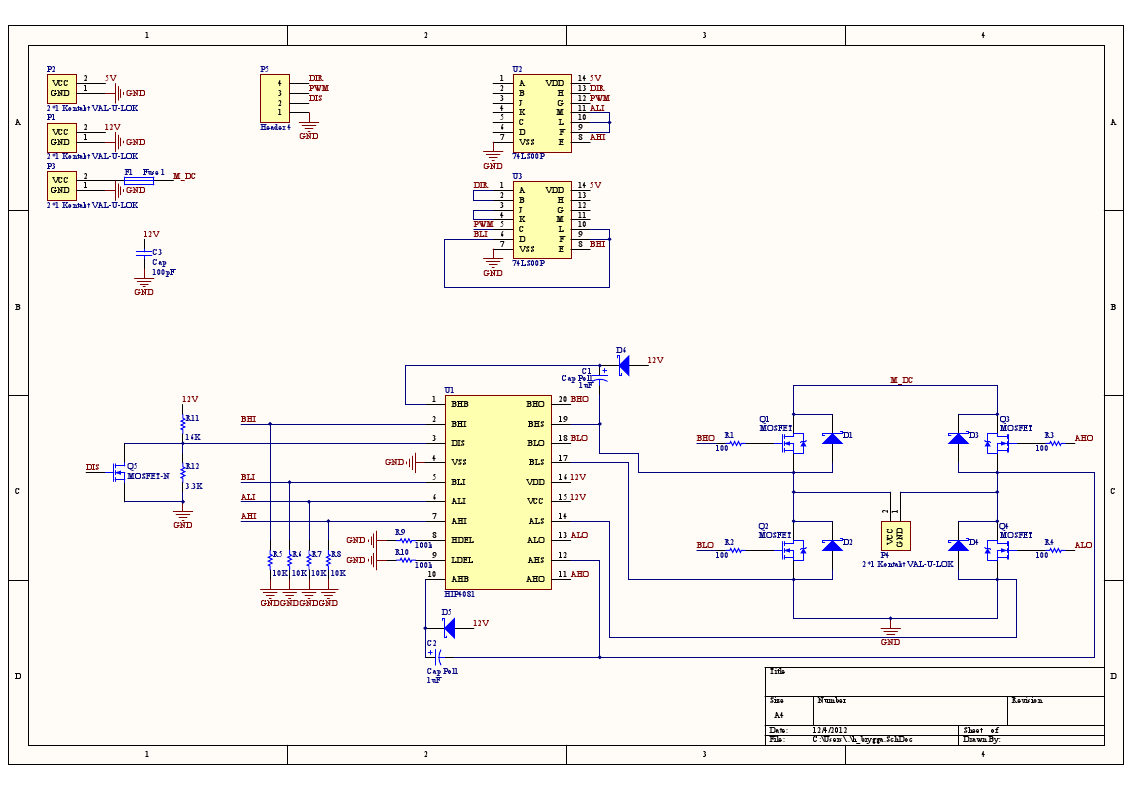
\includegraphics[width=20cm]{../../includes/figures/h_brygga_schematic}
\caption{Kretsschema.}
\label{fig:h_brygga_schema}
\end{figure}
\end{landscape}

PCB-layouten kan ses i figur \ref{fig:pcb_layout}, enbart hålmonterade komponenter användes för att det skulle bli enklare att montera.

\begin{figure}[htbp!]
\centering
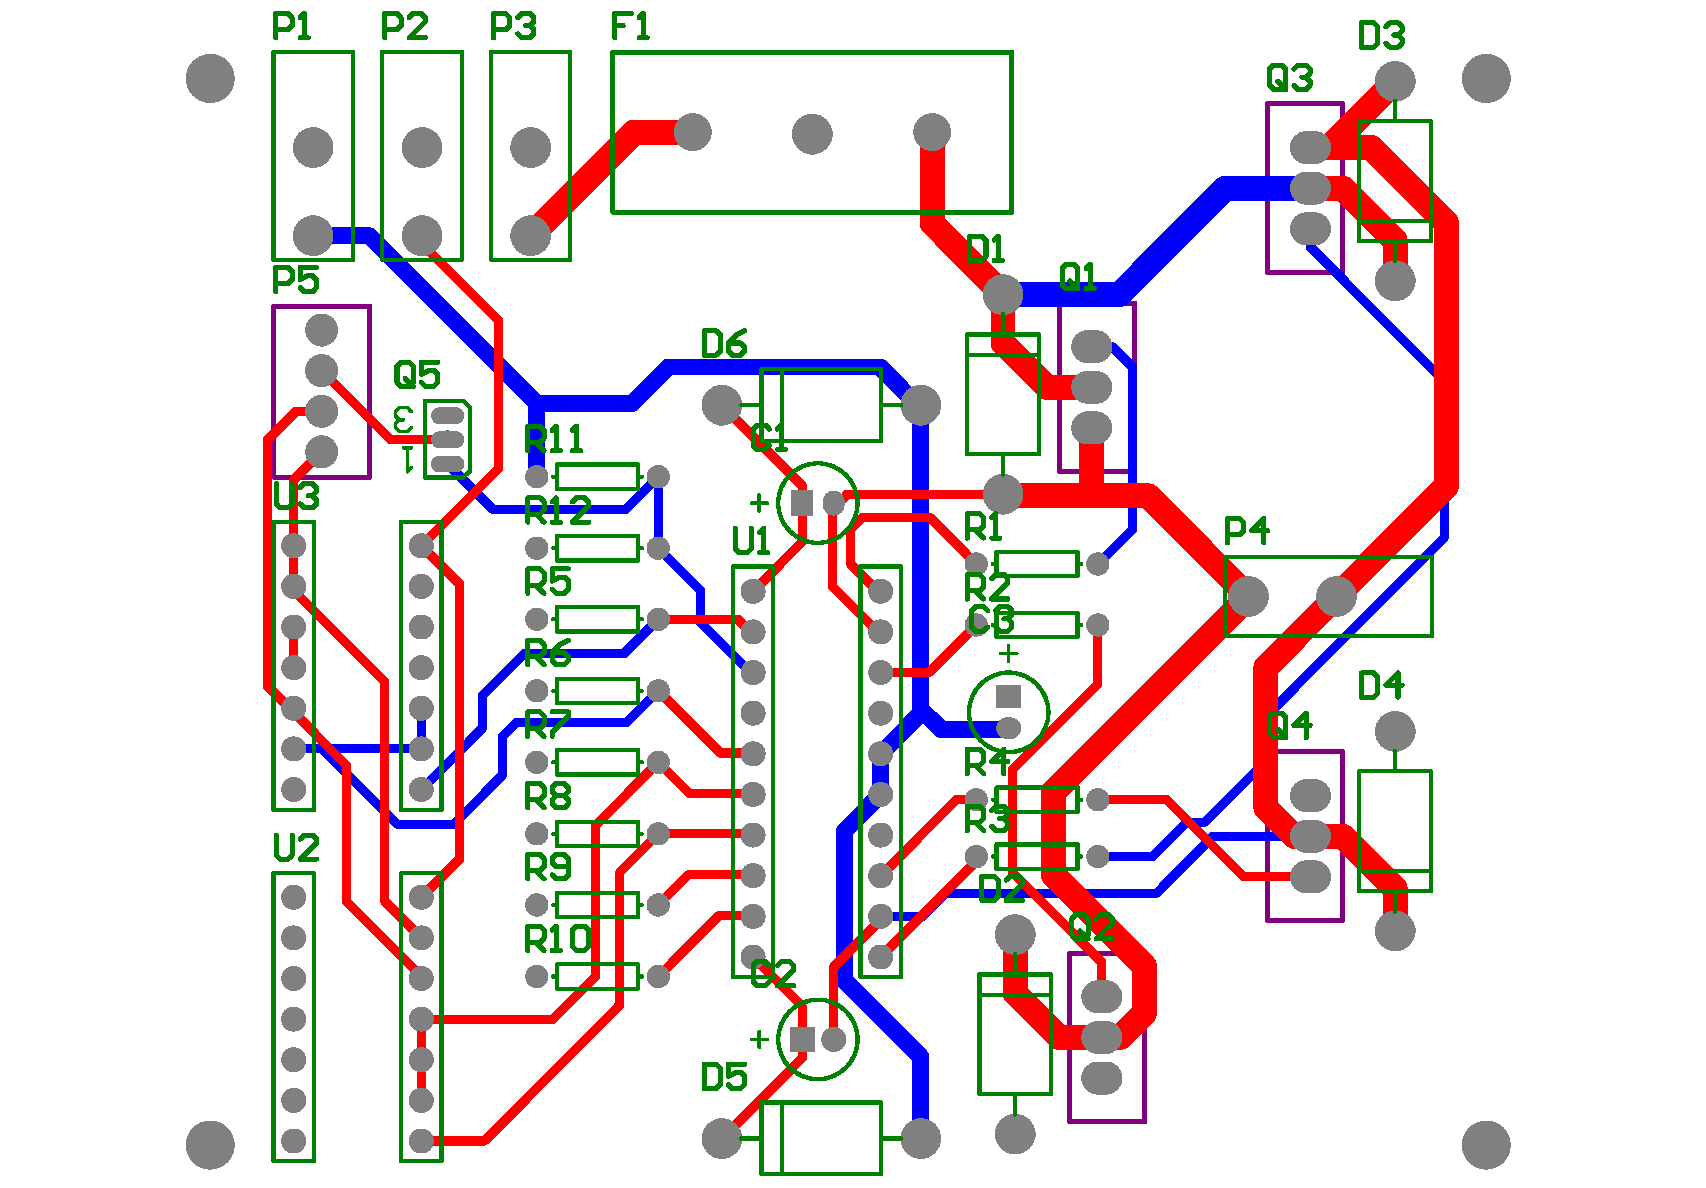
\includegraphics[width=12cm]{../../includes/figures/H_brygga_pcb}
\caption{PCB-layout.}
\label{fig:pcb_layout}
\end{figure}

Den färdiga h-bryggan kan ses i figur \ref{fig:mounted_h_bridge}.

\begin{figure}[htbp!]
\centering
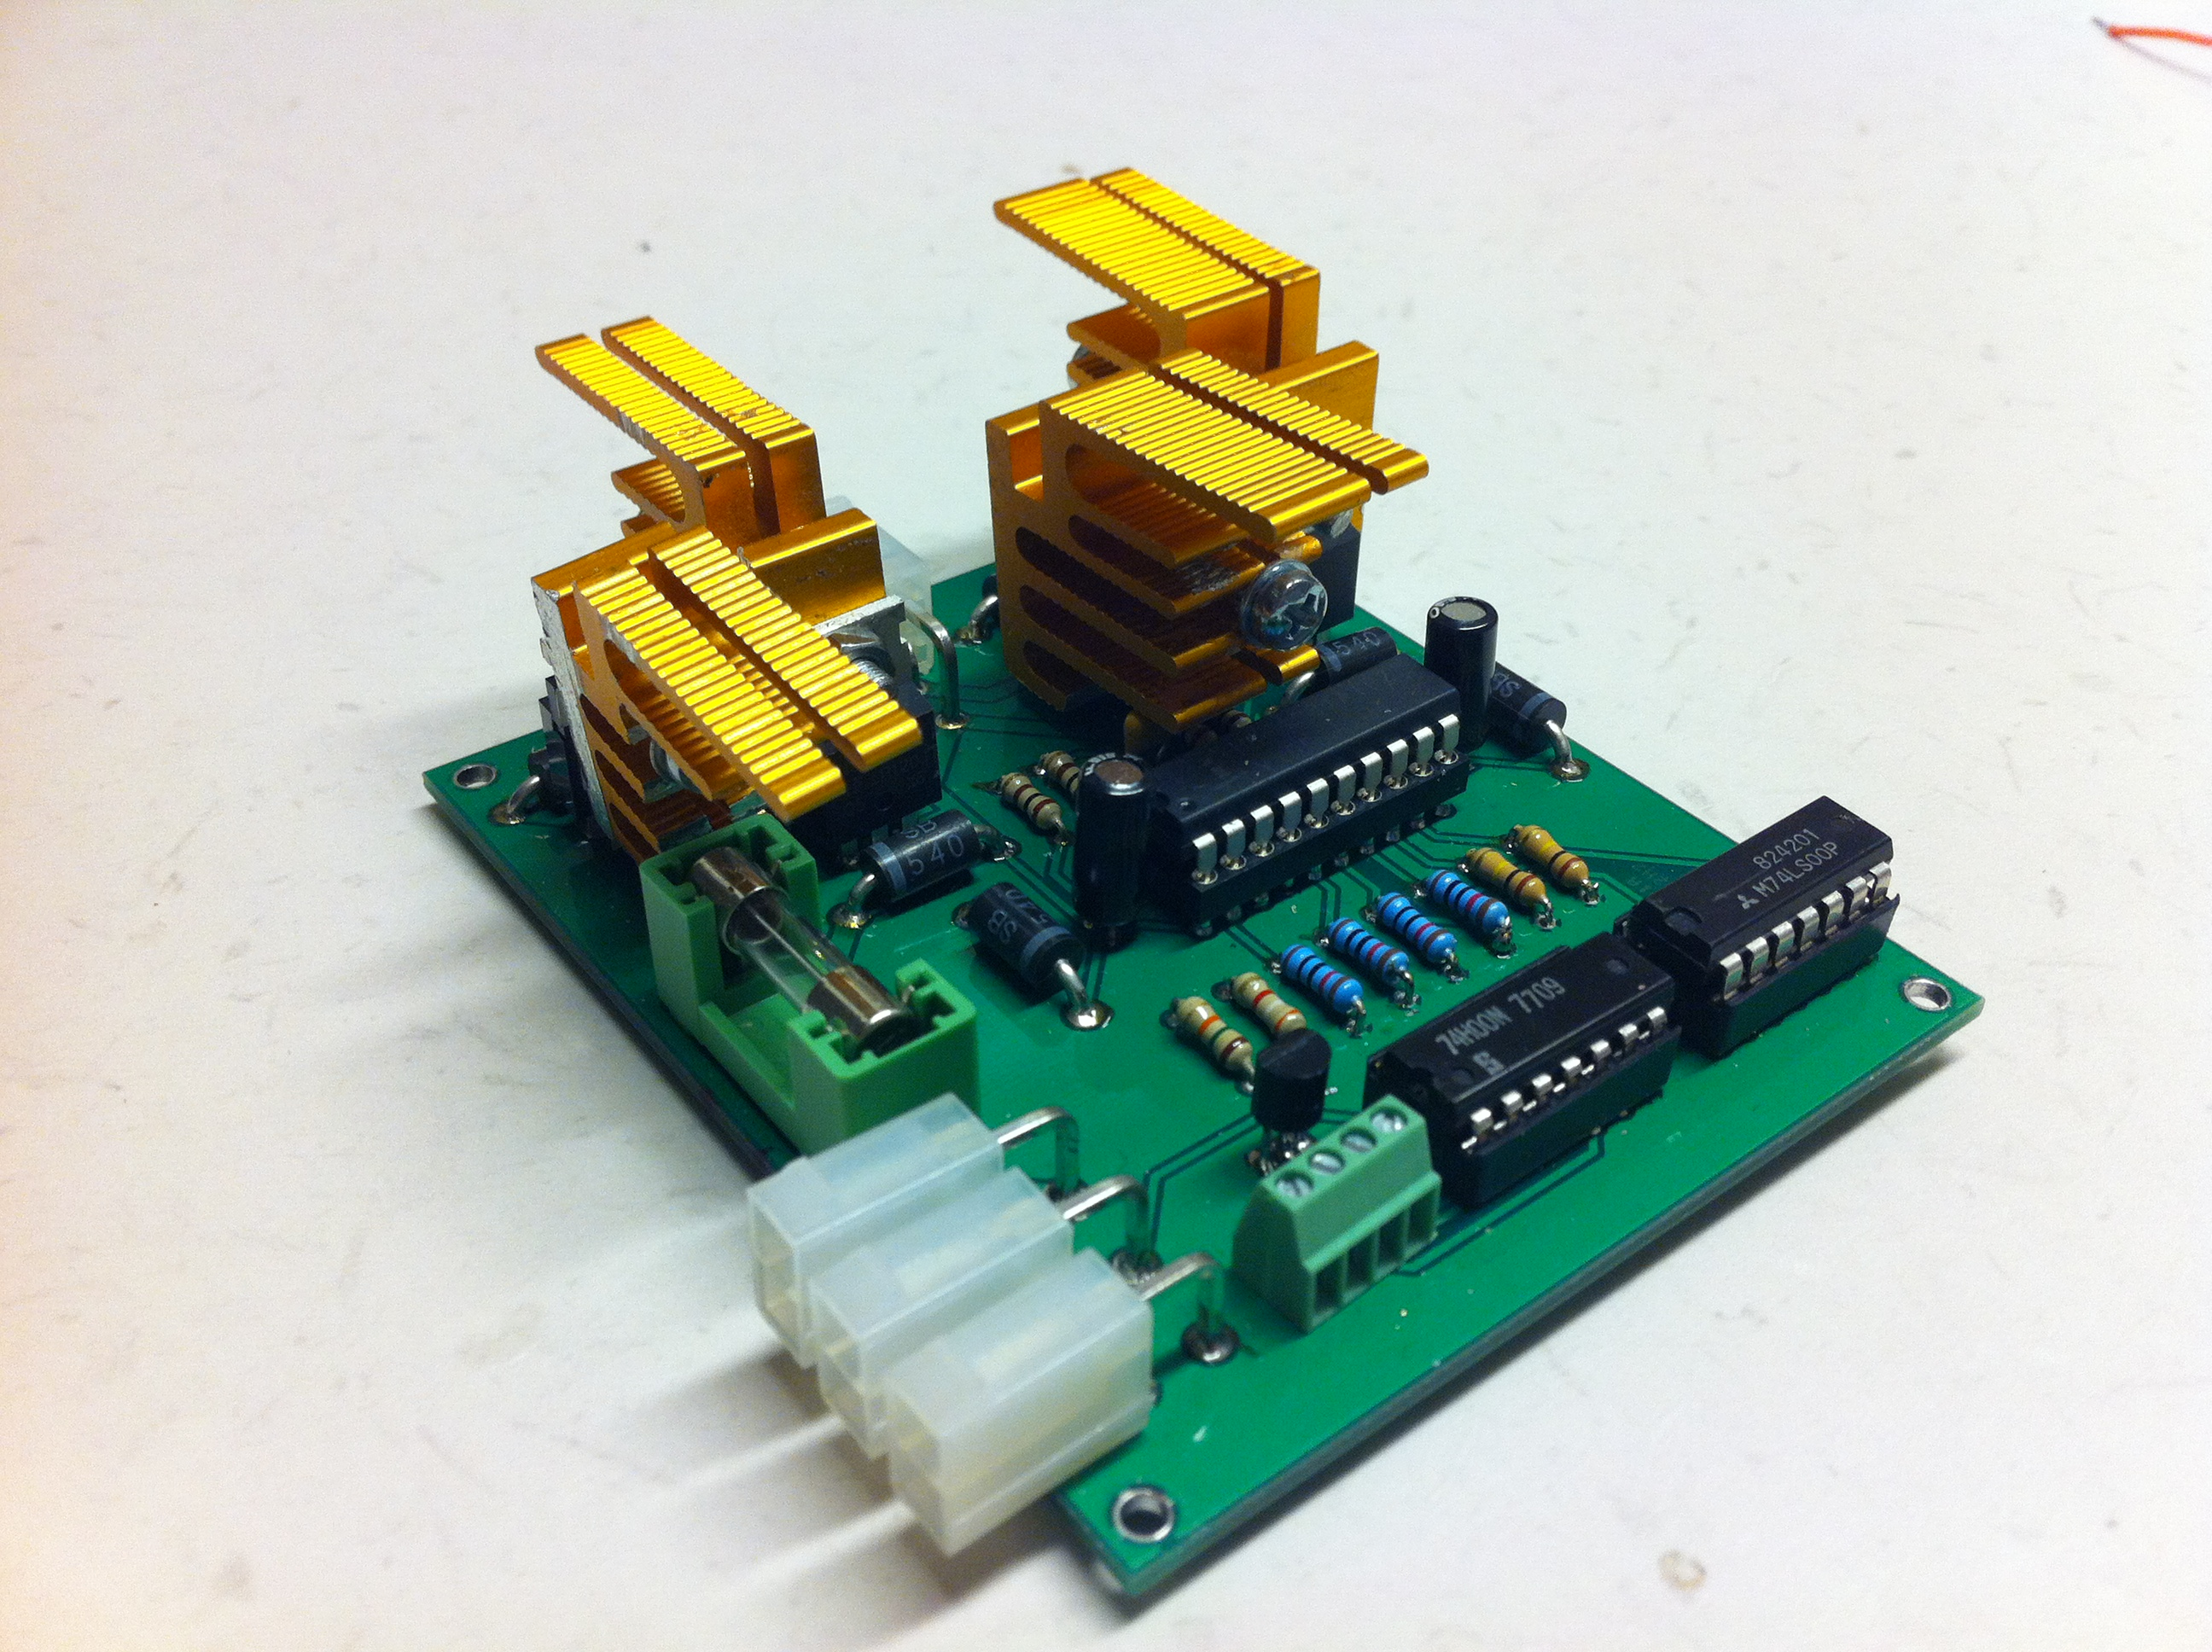
\includegraphics[width=10cm]{../../includes/figures/Hbridge}
\caption{Den färdiga h-bryggan.}
\label{fig:mounted_h_bridge}
\end{figure}

\subsubsection{Diskussion}
H-bryggan fungerade bra och det finns även möjlighet till att styra mer effektkrävande motorer då MOSFET:arna är specade för upp till 55V 110A ifall att en mer kraftfull motor skulle användas.

\subsubsection{Ekonomi}
En tabell över komponenter till en h-brygga ses i tabell \ref{tbl:BOM}, de komponenter som fanns på skolan fick vi gratis därför är de prisatta som 0kr. Den totala kostnaden för två h-bryggors komponenter var 617,88kr. 

\begin{table}[htb]
\centering
\caption{Tabell över komponenter}
\label{tbl:BOM}
\begin{tabular}{|l|l|r|c|c|}
\hline
\textbf{Komponent} & \textbf{Information} & \textbf{Antal} &
\textbf{Notation i schemat} & \textbf{Pris/st} \\
\hline
MOSFET driver & HIP4081AIPZ & 1 & U1 & 102 \\
\hline
Schottky diode & SB340 & 6 & D1-D5 & 4.93\\
\hline
Power MOSFET & IRF3205PBF & 4 & Q1-Q4 & 43.5\\
\hline
Small signal transistor & 2N3906 & 1 & Q5 & 0\\
\hline
Resistor & 100~k$\Omega$ & 2 & R9, R10 & 0\\
\hline
Resistor & 10~k$\Omega$ & 4 & R5-R8 & 0\\
\hline
Resistor & 100~$\Omega$ & 4 & R1-R4 & 0\\
\hline
Resistor & 16~k$\Omega$ & 1 & R11 & 0\\
\hline
Resistor & 3.3~k$\Omega$ & 1 & R12 & 0\\
\hline
Quad 2-input NAND & 7400 & 2 & U2, U3 & 0\\
\hline
Electrolytic capacitor & 1~uF & 2 & C1, C2 & 1.68\\
\hline
Ceramic capacitor & 1~uF & 1 & C3 & 0\\
\hline
Male Connector 90$^{\circ}$ & 2~p & 4 & P1-P4 & 0\\
\hline
PCB Terminal Block &  4~p & 1 & P5 & 0\\
\hline
Fuse holder & 6.7 A & 1 & F1 & 0\\
\hline
\end{tabular}	
\end{table}